\chapter{Basic Notions} 
\label{chap:notions}

To make this work more self-contained, we briefly introduce basic notions and concepts used in the later chapters. 
Interested reader is refferred to the monographs \cite{szeliski2010, multipleview} for further details.

\section{Convolution}

\term{Convolution} is an operation on two functions often encounterred in signal processing.
In image processing, convolution is typically used to apply a particular filter (kernel) to the image.
For example, the output of such convolution can be a blurred image. 
Convolution with a Gaussian kernel is particularly common. 
\begin{definition}
\term{The convolution of functions $f$ and $g$} is an operation defined as:
\begin{align*}
(f \convolution g)(t)&=\inftyint f(\tau)g(t -\tau) d\tau.
\end{align*}
\end{definition} 
In our setting, the $f$ from the above definition represents the image function and $g$ the filter.

\section{Image derivatives}
\label{sec:imder}
\term{Image derivatives} of an image function are analogous to derivatives of a real continuous function.
They allow us to meassure spacial changes in an image by expressing the rate of image intensity change in a particular direction. 
High values often indicate an edge in the image data. 
They are defined as
\begin{align*}
\imd{\partial x}(x, y)& = I(x + 1, y) - I(x-1, y), \\
\imd{\partial y}(x, y)& = I(x, y + 1) - I(x, y - 1),
\end{align*}
where $I$ is the input image and $(x, y)$ are coordinates of the pixel.
A generalization of this is often considered since the above discretization is not able to detect significant intensity changes spread across more than few pixels. 

\subsection{Gaussian image derivatives and scale-space}
\label{sec:gaussder}

Scale-space of an image is a series of gradually more and more smoothed images obtained by convolving the original image with Gaussian kernels of increasing size.
Formally, it is a series of image functions $\L$ defined as the convolution of the image function $\func$ and the Gaussian kernel $\gauss$, where $t$ is the corresponding variance: % XXX nechceme sjednotit to, jestli budeme tu varianci oznacovat jako $t$ nebo $\sigma$? 
%\begin{align*}
%\gauss = \frac{1}{2\pi t} e^{-(x^2+y^2)/2t}
%\end{align*}
\begin{align*}
\L = \func \convolution \gauss.
\end{align*}

To this scale-space representation we can apply local derivatives at any scale.
Equivalently, scale-space derivatives can be computed by convolving the original image $f$ with Gaussian derivative operators which are derivatives of the Gaussian function.
For this reason they are often also referred to as \term{Gaussian derivatives}.

\subsection{Laplacian}

As already mentioned, \term{image derivatives} are useful for the purpose of the detection high variations of image intensity values.
After taking the first derivative of the image function, points of highest intensity change are those where we have local maxima. 
If we go further and take the second derivative, then the corresponding values transform to zeroes.
Thus, it might be important to consider the sum of derivatives in the direction of both axes to detect such structures. 

\begin{definition}
The Laplacian of a function with $n$-dimensional support is the divergence of the gradient of a function $f$:
\begin{align*}
\nabla^{2}f &= \sum_{i=0}^{n} \fpp{ \partial x_i^2 }.
\end{align*}
In image processing we usually consider $2$-dimensional space, thus the \term{Laplacian} becomes: 
\begin{align*}
\nabla ^{2}f(x, y)&=\fpp{\partial x^2} + \fpp{\partial y^2}.
\end{align*}
\end{definition} 

Similar argument to the above can be used to deduce that local maxima and minima of the Laplacian function indicate the presence of a blob-like structure in the image data. 
The size of the structure is related to the variance of the Gaussian used in the definition of the Gaussian image derivatives of Section \ref{sec:gaussder}. 
For this reason, algorithms like SIFT \cite{lowe1999} repeat some parts of the computation for varying values of this parameter to detect structures of all sizes. 

\subsection{Hessian matrix}

% feature detectors and interest points descriptors employ the Hessian matrix of the image.
The Hessian matrix describes a second-order behaviour of a function around a particular point. 

\begin{definition} 
\term{The Hessian matrix of a function $f: \Rn \to \R$ at $\x \in \Rn$} is a matrix $H_f(\x)$ of the second order partial derivatives of $f$ evaluated at $\x$: %~=~(x_1, \ldots, x_n)$: 
\begin{align*} 
H_f(\x) := 
\begin{pmatrix} 
\fpp{ \partial x_1^2 }              &   \fpp{ \partial x_1 \partial x_2 }   &   \ldots   &   \fpp{ \partial x_1 \partial x_n }   \\ 
\fpp{ \partial x_2 \partial x_1 }   &   \fpp{ \partial x_2^2 }              &   \ldots   &   \fpp{ \partial x_2 \partial x_n }   \\ 
\hdotsfor[2]{4} \\ 
\fpp{ \partial x_n \partial x_1 }   &   \fpp{ \partial x_n \partial x_2 }   &   \ldots   &   \fpp{ \partial x_n^2 }  
\end{pmatrix}. 
\end{align*} 
If any of the partial derivatives on the right-hand side are undefined, we say that the Hessian matrix is also undefined.
% \[ H(f, \x) = \left(\begin{array}{c}  
% \frac{\partial^2 f}{\partial x_1^2} \frac{\partial^2 f}{\partial x_1 \partial x_2} 
% \cdots \frac{\partial^2 f}{\partial x_1 \partial x_n}\\
% \frac{\partial^2 f}{\partial x_2 \partial x_1} \frac{\partial^2 f}{\partial x_2^2} 
% \cdots \frac{\partial^2 f}{\partial x_2\partial x_n}\\
% \cdots \cdots \cdots \\
% \frac{\partial^2 f}{\partial x_n \partial x_1} \frac{\partial^2 f}{\partial x_n \partial x_2} 
% \cdots \frac{\partial^2 f}{\partial x_n^2}
% 
% \end{array}\right)  \]
\end{definition} 
Note that the trace of the Hessian matrix is equal to the Laplacian at the same point $\x$. 

Within the context of image processing, the function $f$ typically corresponds to the input image and derivatives are replaced either by differences between the intensity levels of neighbouring pixels or Gaussian derivatives. 

The Hessian matrix forms a basis for a basic feature detector (called Hessian detector), which selects the image positions $\x$ locally maximizing $\det(H(I, \x)),$ where $I$ is the input image.
This leads to a detection of corners and features of size roughly comparable to the variance of the Gaussian kernel used to compute the Gaussian derivatives. % TODO zkontrolovat, jestli to neni nesmysl

\section{Basic image similarity metrics} % XXX zamyslet se nad timhle nazvem a jestli je to skutecne metrika

We now introduce two simple metrics that can be used to estimate similarity of visual contents of a pair of images. 
These are often used as a basis for more sophisticated image registration algorithms, e.g. \cite{hirschmuller2008}.

\term{Sum of absolute differences} describes the difference of intensities of corresponding areas of two images: 
\begin{definition} 
Let $I_1(x, y)$ and $I_2(x, y)$ be two grayscale images. 
Then \term{the sum of absolute differences of $I_1$ and $I_2$} is the value $\sum_{x, y} |I_1(x, y) - I_2(x, y)|$. 
\end{definition} 
Note that this value is going to be zero for a pair of identical images.

For the second metric, % XXX tady je to slovo metric taky 
we need to recall the definition of \term{entropy} (sometimes also called \term{Shannon entropy}). 
It can be viewed as a meassure of information complexity of a random variable. 
\begin{definition} 
The entropy $H$ of a random variable $X$ with probability distribution $P(X)$ is defined as % XXX zkontrolovat, jestli to skutecne je probability distribution 
\begin{align*}
  H(X) = \E[-\log(P(X))] = -\sum_k{P(k)\log P(k)},
\end{align*}
where $\E[\cdot]$ is the expected value operator.
\end{definition}
In \cv, it is used to meassure the ``complexity'' of the image histogram when the underlying random variable is set as $X = I(\x)$, where $\x$ is a uniformly randomly generated image position. 
A constant, uniform image attains minimum entropy while random noise maximizes it. 

We can now introduce the \term{mutual information} of two images. 
Generally, it measures the mutual dependence of two variables. 
It expresses how much the value of one random variable predicts the value of the other.
\begin{definition}
\term{The mutual information} of two variables $I_1$ and $I_2$ is defined as
\begin{align*}
\MI{I_1, I_2} = & \H{I_1} + \H{I_2} - \H{I_1, I_2},
\end{align*}  
where $H_{I_1, I_2}$ is the entropy $H(X)$, where $X = (I_1(\x), I_2(\x))$ for $\x$ uniformly random. 
In the context of \cv, the vector $\x$ is a random image position. 
\end{definition}
We can also interpret \term{mutual information} as a reduction of uncertainty of one random variable given the knowledge of another.
High mutual information indicates a large reduction in uncertainty and vice versa. 
Mutual information of two images depends only on their joint histogram. 
Again, this value attains zero for a pair of identical images. 
However, it remains zero even after, e.g., increasing the brightness of one of the images. 
Thus, this meassure is invariant under illumination changes, which is of great importance when matching photos taken in an uncontrolled environment. 

\section{Projective geometry}

In the standard Euclidean space $\R^n$, the infinity does not exist.
However, many geometric concepts are simplified when the notion of infinity is included.
An example of such a geometry is \term{the projective geometry}.
Projective plane $\P^2$, or generally projective space $\P^n, n \in \N$, is obtained by extending $\R^n$ by including a point at infinity for each direction.

Numerically, the points in $\P^n$ are represented using non-zero vectors from $\R^{n+1}$.
Suppose we have a point $(x, y)$ in the Euclidean plane.
This point in projective geometry is expressed by the vector $(x, y, 1)$ and any of its non-zero multiples $k \cdot (x, y, 1), k \neq 0$.
These are called \term{homogenous coordinates} of the point.
In what follows, we identify the point in a projective space with the vector of its homogeneous coordinates. 
To get back the Euclidean coordinates we simple divide the first two coordinates by the third.
We can notice that none of the points $(x, y)$ from Euclidean space corresponds to a projective point of the form $(x, y, 0)$, because the operations $\frac{x}{0}$ and $\frac{y}{0}$ are undefined.
Such non-zero vectors are used to represent the points at infinity, with each corresponding to a particular direction. 

Similarly to points, lines in the projective plane can also be modelled as non-zero $(n + 1)$-dimensional real vectors. 
A point lies on a line if the dot-product of the corresponding vectors is zero. 
It can be easily seen that the line $k \cdot (0, 0, 1), k \neq = 0$ contains all the points at infinity and is therefore termed \term{the line at infinity}. 
In higher dimensions, lines generalize to planes and hyper-planes. 
The question of representing lines in $\P^3$ is more subtle; we refer the reader to an overview of different approaches in \cite{multipleview}. % XXX pridat do citace specifikaci konkretnich stran

From the perspective of \cv, the most important property of projective geometry is that it allows us to express the projective camera using linear algebra. 
This makes it possible to build on the grounds of this well-understood area.

\term{Projective camera} represents a model of central perspective projection.
It maps points from $\P^3$ (world) to $\P^2$ (image).
In Figure \ref{fig:camera} we can see the camera geometry.
There, the \term{camera centre} is positioned at the coordinate origin, while the image plane is in front of the camera.
The line perpendicular to the \term{image plane} with one end-point in the centre is called \term{the principal axis} of the camera and its intersection with the image plane is \term{the principal point}.
The world point is projected by intersecting a ray going through the camera center and the world point with the image plane. 
This mapping from $\P^3$ to $\P^2$ can be algebraically expressed as multiplication with a real $3 \times 4$ matrix $\Proj$. 
Note that the overall scale of the matrix does not affect the result. 
Thus, the matrices $k \cdot \Proj, k \neq 0$ represent the same camera. % XXX mozna bysme mohli na odpovidajici mista hodit odkazy do MVG knizky 

The simple algebraic model of the action of the projective camera on the world points is the main strength of concept. 
However, it cannot model some properties of physical cameras applied in practice. 
Most importantly, non-linear distortion of the image (e.g., barell distortion) cannot be modeled by a projective camera. 

%\begin{align*}
%\begin{bmatrix}
 % x_1\\
  %x_2\\
  %x_3
%\end{bmatrix}&= 
%\T
%\begin{bmatrix}
 % X_1\\
  %X_2\\
  %X_3\\
  %X_4
%\end{bmatrix},
%\end{align*}
%where $\T$ is the transformation from homogenous coordinates to Euclidean space.
\begin{figure}[h]
  \label{fig:camera}
  \centering{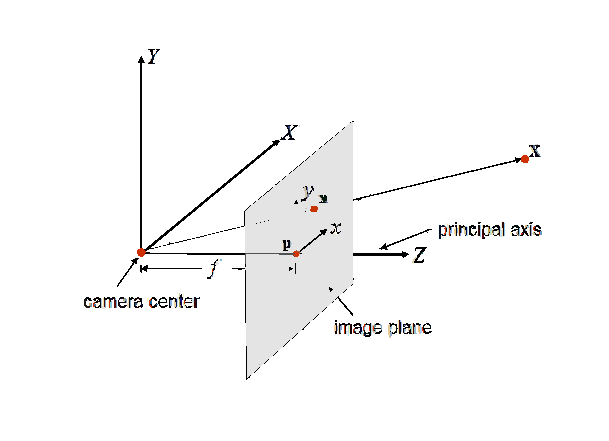
\includegraphics[width=96mm]{img/perspectivecamera.png}}
  \caption{\todo{tento obrazek jsem stahla z googlu, mel by se nahradit}} % XXX tohle musime zmenit 
\end{figure}

\subsection{Epipolar geometry}
\label{sec:epi}

% In \cv\ \term{fundamental matrix} represents the relation of points between two stereo images.
Epipolar geometry expresses the geometric constraints encountered when observing a 3D scene by a pair of cameras with known parameters. 
Suppose we choose a point $\x$ on the image of the first camera from such a pair.
The knowledge of its position constraints the position of the corresponding one on the second image.
This point, denoted by $\xd$, lies on the line $\F\x$, where $\F$ is the fundamental matrix.
This line is called \term{the epipolar line}.

\begin{definition}
The \term{fundametal matrix $\F$} for a pair of stereo images is a $3 \times 3$ matrix which satisfies 
\begin{align*}
\xd^T \F \x = 0
\end{align*}
for any pair of corresponding points $\x$ and $\xd$.
\end{definition}

Fundamental matrix for a pair of photos can be estimated from the knowledge of a set of corresponding points since each correspondence is a linear constraint on the values of $\F$. 
Because $\F$ has $9$ real entries and is determined only up to a scaling factor, it has $8$ degrees of freedom and thus at least $8$ correspondences are required to determine its values. 
However, in our case, the matrix is going have only one degree of freedom due to the restrictions we have specified for the input photographs. 
% Since automatic image registration algorithms typically produce more than $8$ correspondences, this

\section{Integral images}

% Later in this work we work with the term of integral images. 
\term{An integral image}, also known as \term{summed area table}, allows fast and efficient computation of a sum of image intesity values inside an arbitrary rectangular area.
A pixel of an integral image represents the sum of all of the original image's pixels that lie to the left and above the considered position: 
\begin{equation*}
\K_I(\x) := \sum_{i \le x} \sum_{j \le y} I(i,j),
\end{equation*}
where $\K$ is the resulting integral image, \emph{I} is the input image image, and $\x = \vect{(x, y)}^{T}$ is a location of a pixel.

An advantage of the integral image is that we are able to compute it using only one pass through the original image. 
Moreover, once we have calculated the integral image, only three integer operations and four memory accesses are required to calculate the sum 
of the original intensities inside any rectangular region (see Figure \ref{fig:integral}).

\begin{figure}[h]
  \label{fig:integral}
  \centering{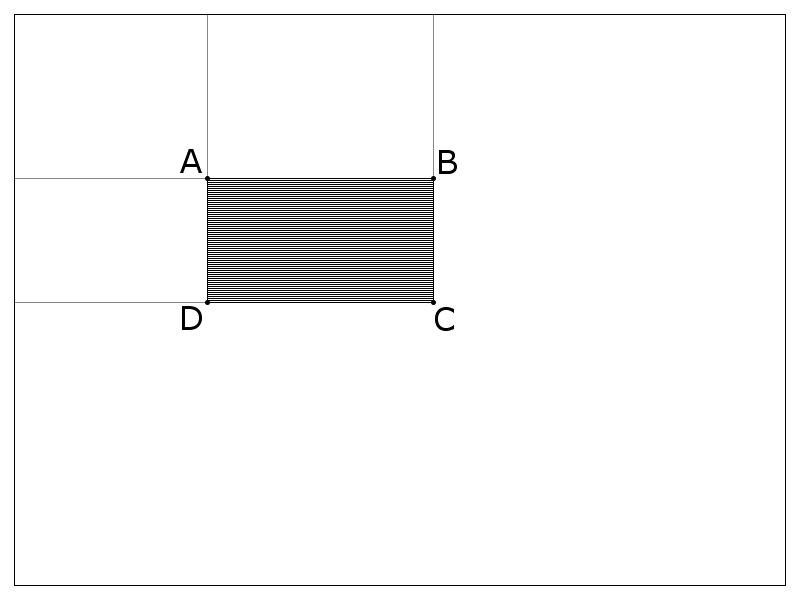
\includegraphics[width=96mm]{img/integral_image.png}}
  \caption{The sum of any rectangular region can be calculated by only three additions: $\sum = C - D - B + A$.}
 \end{figure}




% XXX nedat sem nekam jeste neco o tom, jak vypocitat hloubku z disparity?
